%%%%%%
%
% $Autor: Wings $
% $Datum: 2020-01-18 11:15:45Z $
% $Pfad: githubtemplate/Template/Presentations/Template/slides/rename.tex $
% $Version: 4620 $
%
%
% !TeX encoding = utf8
% !TeX root = Rename
%
%%%%%%



%%%%%%%%%%%%%%%%%%%%%%%%%%%%%%%%%%%%%%%%%%%%%%%%%%%%%%%%
%%%%%%%%%%%%%%% SYSTEM OVERVIEW %%%%%%%%%%%%%%%%%%%%%%%%
%%%%%%%%%%%%%%%%%%%%%%%%%%%%%%%%%%%%%%%%%%%%%%%%%%%%%%%%

\Mysection{System Overview}

\STANDARD{Mobile Robot Architecture}{
\begin{itemize}
  \item Compute: NVIDIA Jetson Nano Developer Kit
  \item Cameras: Raspberry Pi HQ / CS / V2
  \item Locomotion: 4× TT motors + metal caster
  \item Control: Qwiic motor driver
  \item Feedback: Qwiic OLED status display
  \item Communication: 433 MHz antenna
  \item Wiring: Qwiic cable ecosystem
\end{itemize}


\begin{figure}
	\centering
	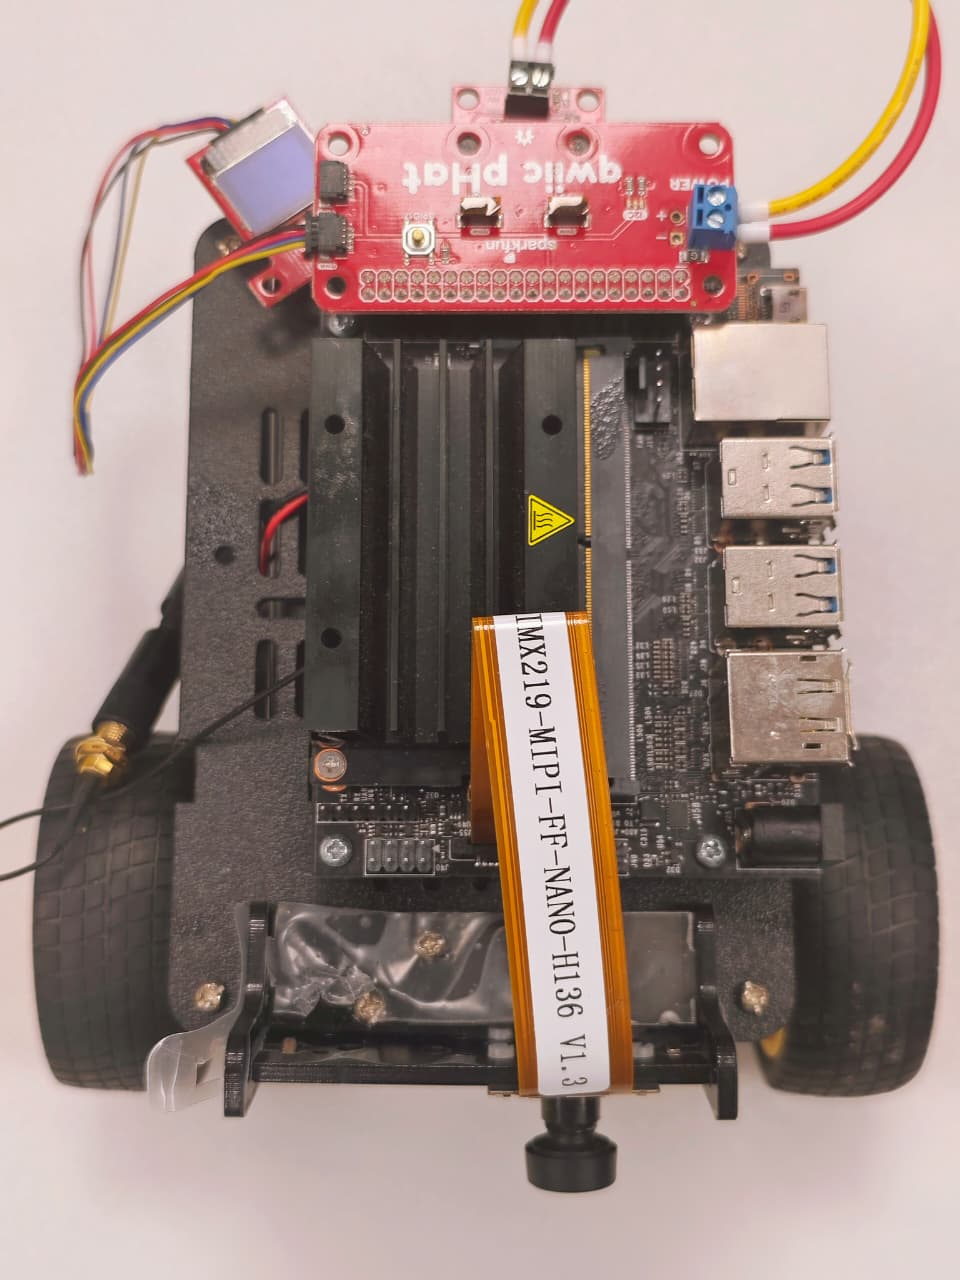
\includegraphics[width=0.4\linewidth]{images/MBTopView}
	\caption{Mobile Robot Top View}
	\label{fig:mbtopview}
\end{figure}
}
\STANDARD{Mobile Robot}{
\begin{center}
\begin{tikzpicture}
  \node (jetson) [rectangle, draw] {Jetson Nano};
  \node (cam) [rectangle, draw, above=1.4cm of jetson] {Camera};
  \node (mot) [rectangle, draw, below=1.4cm of jetson] {Motor Driver};
  \node (ch) [rectangle, draw, below=1.4cm of mot] {Chassis + Motors};
  \node (oled) [rectangle, draw, right=1.4cm of jetson] {Qwiic OLED};
  \node (ant) [rectangle, draw, left=1.4cm of jetson] {433 MHz Antenna};
  \draw[<->] (cam) -- (jetson);
  \draw[<->] (ch) -- (mot);
  \draw[<->] (mot) -- (jetson);
  \draw[<->] (oled) -- (jetson);
  \draw[<->] (ant) -- (jetson);
  
\end{tikzpicture}
\end{center}
}

%%%%%%%%%%%%%%%%%%%%%%%%%%%%%%%%%%%%%%%%%%%%%%%%%%%%%%%%
%%%%%%%%%%%%%%% OS INSTALLATION %%%%%%%%%%%%%%%%%%%%%%%%
%%%%%%%%%%%%%%%%%%%%%%%%%%%%%%%%%%%%%%%%%%%%%%%%%%%%%%%%

\Mysection{Jetson OS Installation}

\STANDARD{Install JetPack on Jetson}{
Compute module: \href{https://www.seeedstudio.com/Jetson-10-1-A0-p-5336.html}{Jetson 10-1 A0 (Jetson Nano)}.
\textbf{Steps:}
\begin{itemize}
  \item Install NVIDIA SDK Manager on a Linux PC
  \item Select Jetson Nano target and JetPack version
  \item Flash image to SD card (using SDK Manager)
  \item Insert SD card into Jetson, connect power, HDMI, keyboard
  \item On first boot: complete Ubuntu setup and enable networking
\end{itemize}
\textbf{Robot software stack:}
\begin{itemize}
  \item Install Python 3, OpenCV, and ROS2 (e.g. Humble) on Jetson
  \item Clone project repository containing \texttt{MR.py}
\end{itemize}
}

%%%%%%%%%%%%%%%%%%%%%%%%%%%%%%%%%%%%%%%%%%%%%%%%%%%%%%%%
%%%%%%%%%%%%%%% PART DETAILS %%%%%%%%%%%%%%%%%%%%%%%%%%%
%%%%%%%%%%%%%%%%%%%%%%%%%%%%%%%%%%%%%%%%%%%%%%%%%%%%%%%%

\Mysection{Part Details: Compute and Cameras}

\STANDARD{Compute: Jetson Nano}{
\href{https://www.seeedstudio.com/Jetson-10-1-A0-p-5336.html}{NVIDIA Jetson Nano Developer Kit(J1010)}:
\textbf{Key features:}
\begin{itemize}
  \item Quad-core ARM CPU + NVIDIA GPU for vision
  \item CSI ports for camera modules
  \item 40-pin header for GPIO / I\textsuperscript{2}C / UART
  \item Boots Ubuntu with JetPack
\end{itemize}
\textbf{Role in robot:}
\begin{itemize}
  \item Runs MR.py and ROS2 nodes
  \item Processes images and computes odometry
  \item Sends motor commands and reads sensors via Qwiic
\end{itemize}
}
\STANDARD{Leopard Imaging LI-IMX219-MIPI-FF-NANO Camera}
{
	\begin{itemize}
		\item \textbf{Module Part Number:} LI-IMX219-MIPI-FF-NANO
		\item \textbf{Compatible Platform:} NVIDIA Jetson Nano Developer Kit
		\item \textbf{Module Size:}
		\begin{enumerate}
			\item H90: 150.0 mm (L) × 25.0 mm (W) × 15.27 mm (H)
			\item H136: 150.0 mm (L) × 25.0 mm (W) × 15.3 mm (H)
			\item H145: 150.0 mm (L) × 25.0 mm (W) × 14.1 mm (H)
		\end{enumerate}
		\item \textbf{Sensor Type:} Sony IMX219, 8.08 MP color
		\item \textbf{Active Pixels:} 3280 (H) × 2464 (V)
		\item \textbf{Optical Format / Diagonal:} Type 1/4.0, 4.60 mm
		\item \textbf{Aperture (F/No):}
		\begin{enumerate}
			\item H90: F/2.6
			\item H136: F/2.0
			\item H145: F/2.5
		\end{enumerate}
		\item \textbf{Focal Length:}
		\begin{enumerate}
			\item H90: 2.3 mm
			\item H136: 1.58 mm
			\item H145: 1.55 mm
		\end{enumerate}
	\end{itemize}
}
\STANDARD{Leopard Imaging LI-IMX219-MIPI-FF-NANO Camera}
{
\begin{figure}
	\centering
	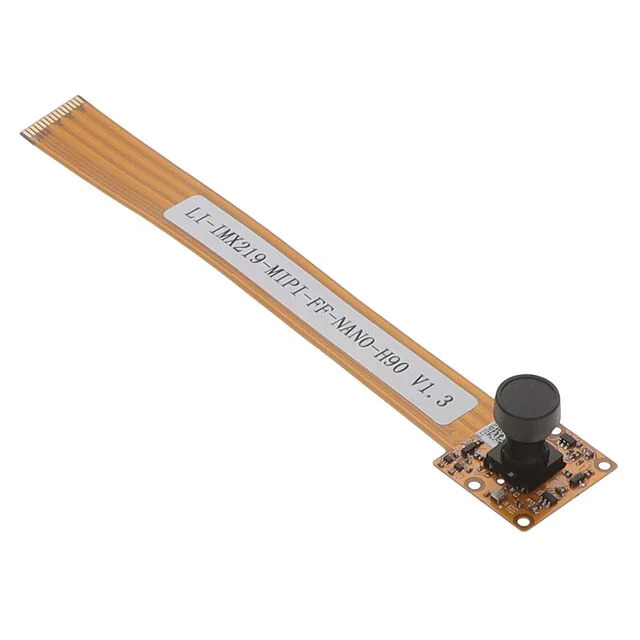
\includegraphics[width=0.5\linewidth]{../images/LIIMX219}
	\caption{Leopard Imaging LI-IMX219-MIPI-FF-NANO Camera}
	\label{fig:liimx219}
\end{figure}
}



\STANDARD{Other Specifications of Leopard Imaging LI-IMX219-MIPI-FF-NANO Camera}{
	\begin{itemize}
		\item \textbf{Horizontal Field of View (FOV):} 90°, 136°, 145°
		\item \textbf{TV Distortion:} < -10% (H90), < -15% (H136/H145)
		\item \textbf{Focusing Range:} 30 cm to infinity
		\item \textbf{Pixel Size:} 1.12 µm × 1.12 µm
		\item \textbf{IR Cut Filter:} Yes
		\item \textbf{Operating Temperature:} -20°C to +60°C
		\item \textbf{Storage Temperature:} -30°C to +80°C
		\item \textbf{Data Output Interface:} CSI-2 MIPI (2-lane)
		\item \textbf{Maximum Image Transfer Rate:} 3280 × 2464 @ 21 fps
		\item \textbf{Mating Connector:} Part No. 1-1734248-5, 15 positions, 1.00 mm pitch
	\end{itemize}
}
\STANDARD{Raspberry Pi HQ Camera}{
Camera: \href{https://www.reichelt.de/de/de/shop/produkt/raspberry_pi_-_kamera_12mp_75_c-_cs-fassung-276919}{12MP HQ Camera}  
Lenses:
\begin{itemize}
  \item \href{https://www.berrybase.de/8-50mm-zoom-objektiv-c-mount}{8--50 mm C-mount zoom lens}
  \item \href{https://www.berrybase.de/en/raspberry-pi-hq-camera-usb-webcam-bundle}{HQ Camera USB Webcam Bundle}
\end{itemize}

\begin{figure}
	\centering
	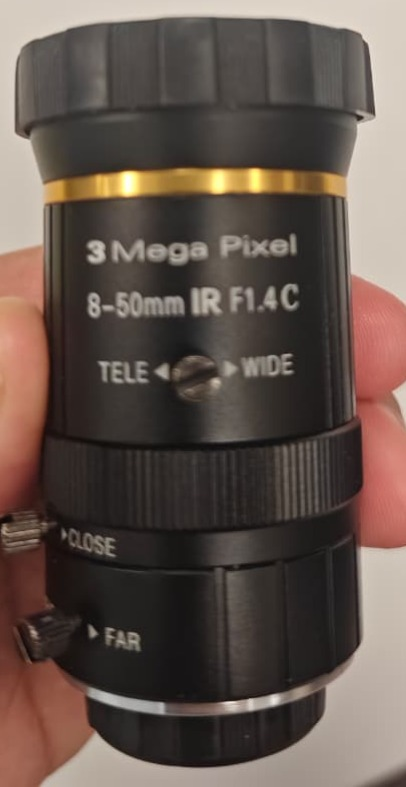
\includegraphics[width=0.3\linewidth]{images/CCTVLENS3MPCMount}
	\caption{CCTVLENS 3MP Camera Mount}
	\label{fig:cctvlens3mpcmount}
\end{figure}

\begin{figure}
	\centering
	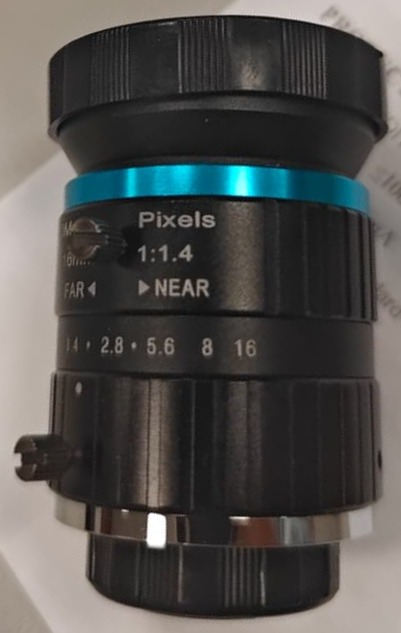
\includegraphics[width=0.2\linewidth]{images/RaspPiHQCam10MPCmount}
	\caption{Raspberry PI HQ Cam Mount 10MP}
	\label{fig:rasppihqcam10mpcmount}
\end{figure}

\begin{figure}
	\centering
	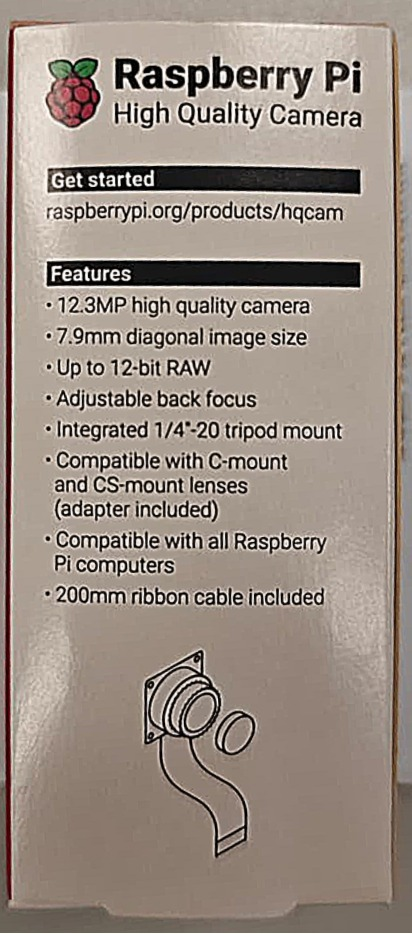
\includegraphics[width=0.2\linewidth]{images/RaspPiHQCamCover}
	\caption{Raspberry Pi HQ Camera Lens Specifications}
	\label{fig:rasppihqcamcover}
\end{figure}

\textbf{Details:}
\begin{itemize}
  \item High resolution, good for mapping and localization
  \item C/CS mount supports interchangeable lenses
  \item Connects via CSI ribbon to Jetson
\end{itemize}
}

\STANDARD{Raspberry Pi CS Camera}{
Camera: \href{https://www.reichelt.de/de/de/shop/produkt/raspberry_pi_-_kamera_1_6mp_shutter_c-_cs-fassung-345205}{1.6MP global shutter C/CS camera}  
Lens: \href{https://www.berrybase.de/en/16mm-telephoto-lens-c-mount}{16 mm telephoto lens}

\begin{figure}
	\centering
	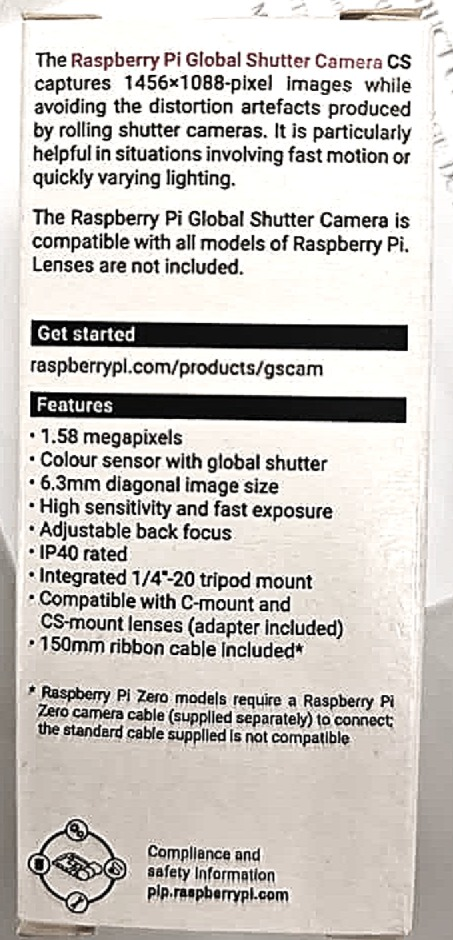
\includegraphics[width=0.2\linewidth]{images/RaspCamGSCover2}
	\caption{Raspberry CamGS Specifications}
	\label{fig:raspcamgscover2}
\end{figure}



\begin{figure}
	\centering
	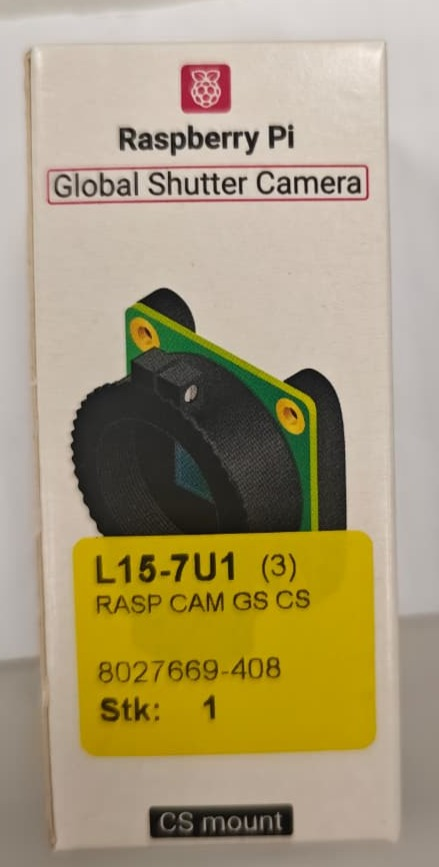
\includegraphics[width=0.2\linewidth]{images/RASPCAMGSCover}
	\caption{Raspberry Pi Cam GS Cover}
	\label{fig:raspcamgscover}
\end{figure}

\footnote{Details:
\begin{itemize}
  \item Global shutter for fast motion scenes
  \item Telephoto lens for distant feature tracking
  \item Same CSI connection method to Jetson
\end{itemize}
}}

\STANDARD{Raspberry Pi Camera V2}{
Camera: \href{https://www.reichelt.de/de/de/shop/produkt/raspberry_pi_-_kamera_8mp_67_v2-170853}{8MP Camera V2}  
Flex cable: \href{https://www.berrybase.de/flexkabel-fuer-raspberry-pi-zero-und-kameramodul/laenge-15-cm}{15 cm flex cable}

\begin{figure}
	\centering
	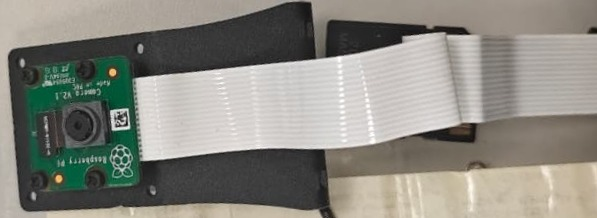
\includegraphics[width=0.7\linewidth]{images/RaspPiCamv2}
	\caption{Raspberry Pi Cam V2 8MP}
	\label{fig:rasppicamv2}
\end{figure}

\begin{figure}
	\centering
	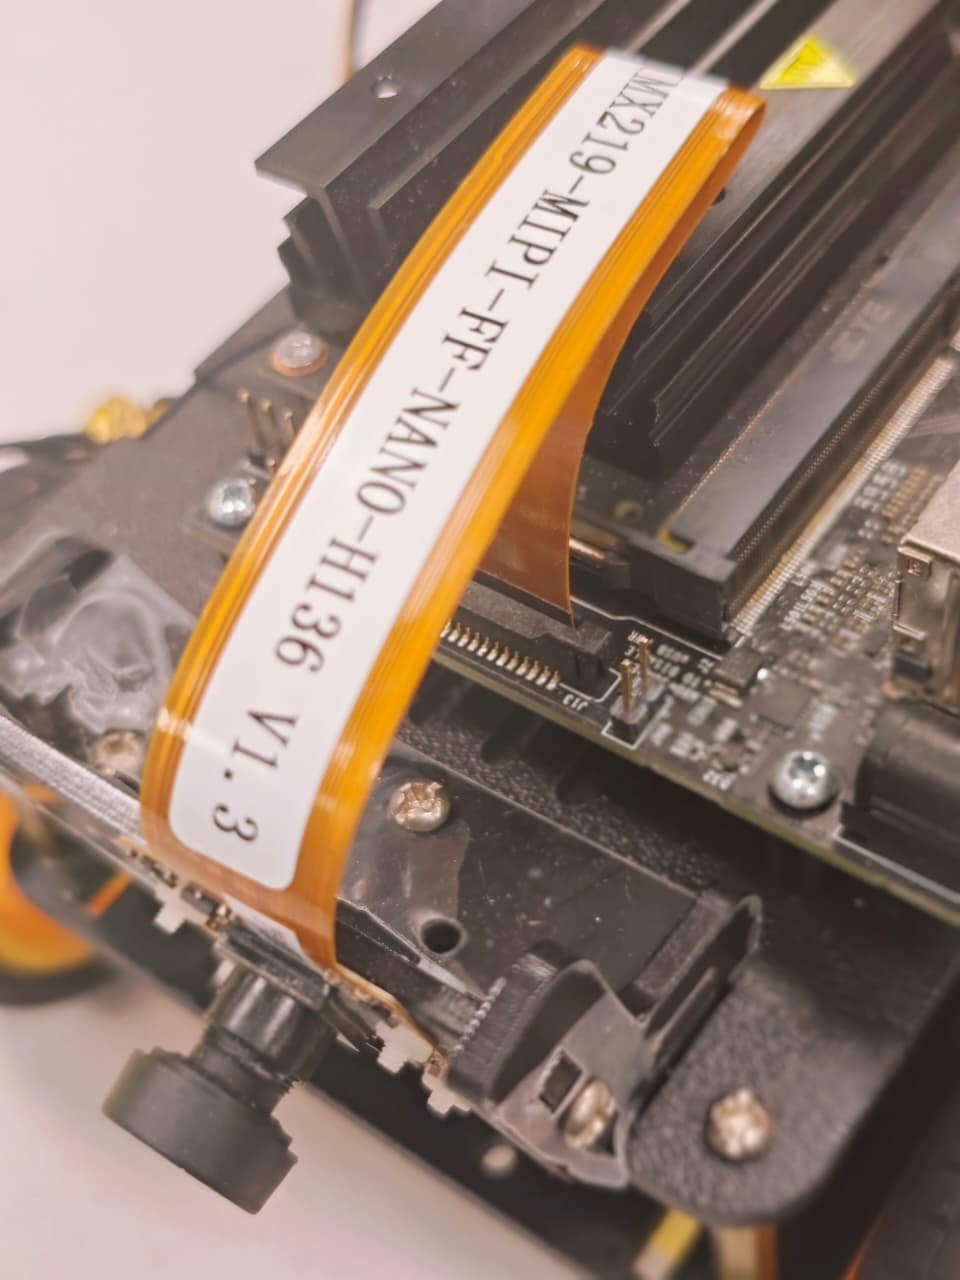
\includegraphics[width=0.4\linewidth]{images/MBFlexcable}
	\caption{Flexible Cable for Camera}
	\label{fig:mbflexcable}
\end{figure}

\textbf{Details:}
\begin{itemize}
  \item Lightweight, compact module
  \item Good for navigation view
  \item Mounted with flex cable to front of chassis
\end{itemize}
}

%%%%%%%%%%%%%%%%%%%%%%%%%%%%%%%%%%%%%%%%%%%%%%%%%%%%%%%%
%%%%%%%%%%%%%%% PART DETAILS: MECHANICS %%%%%%%%%%%%%%%
%%%%%%%%%%%%%%%%%%%%%%%%%%%%%%%%%%%%%%%%%%%%%%%%%%%%%%%%

\Mysection{Part Details: Mechanics}

\STANDARD{Chassis and Wheels}{
Main chassis: Waveshare 2x TT motor chassis

\textbf{Contents:}
\begin{itemize}
  \item Metal base plate
  \item 2× TT DC motors with wheels
  \item Shock-absorbing mounting for rough floors
\end{itemize}

\begin{figure}
	\centering
	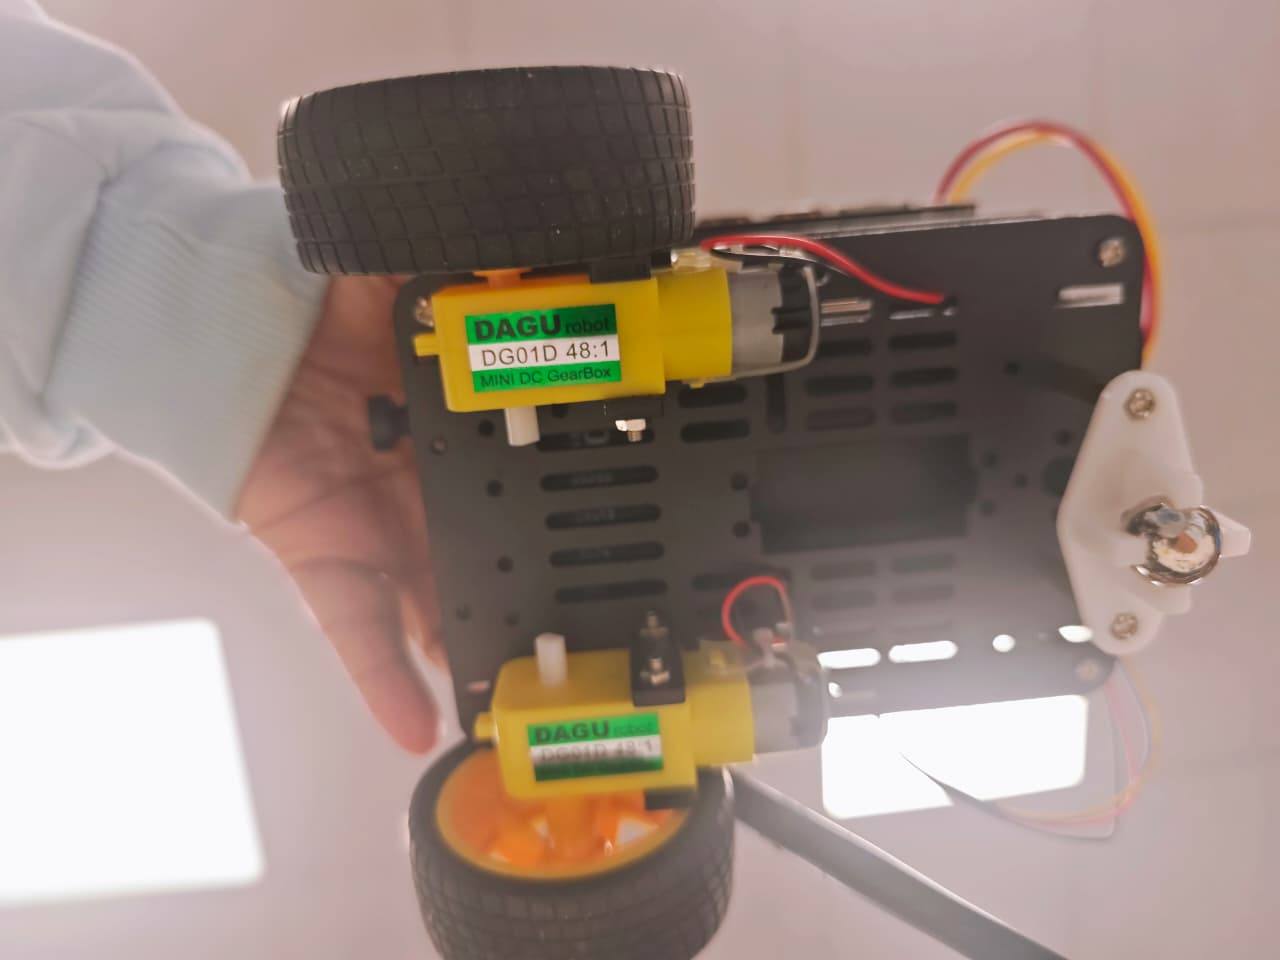
\includegraphics[width=0.7\linewidth]{images/MBBottomView}
	\caption{Mobile Robot Chassis}
	\label{fig:mbbottomview}
\end{figure}

\begin{figure}
	\centering
	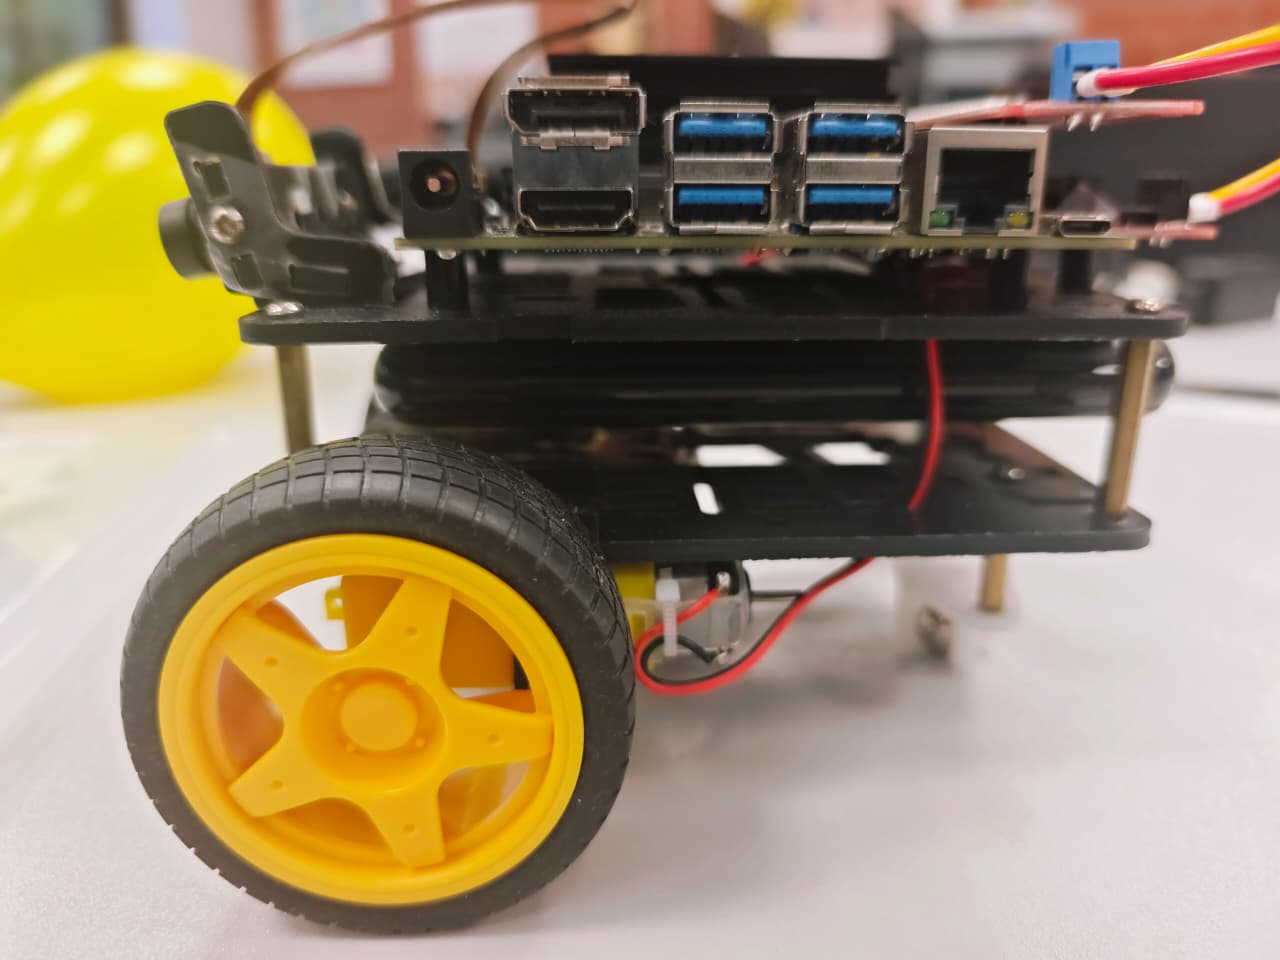
\includegraphics[width=0.7\linewidth]{images/MBSideView}
	\caption{Mobile Robot Side View}
	\label{fig:mbsideview}
\end{figure}

\begin{figure}
	\centering
	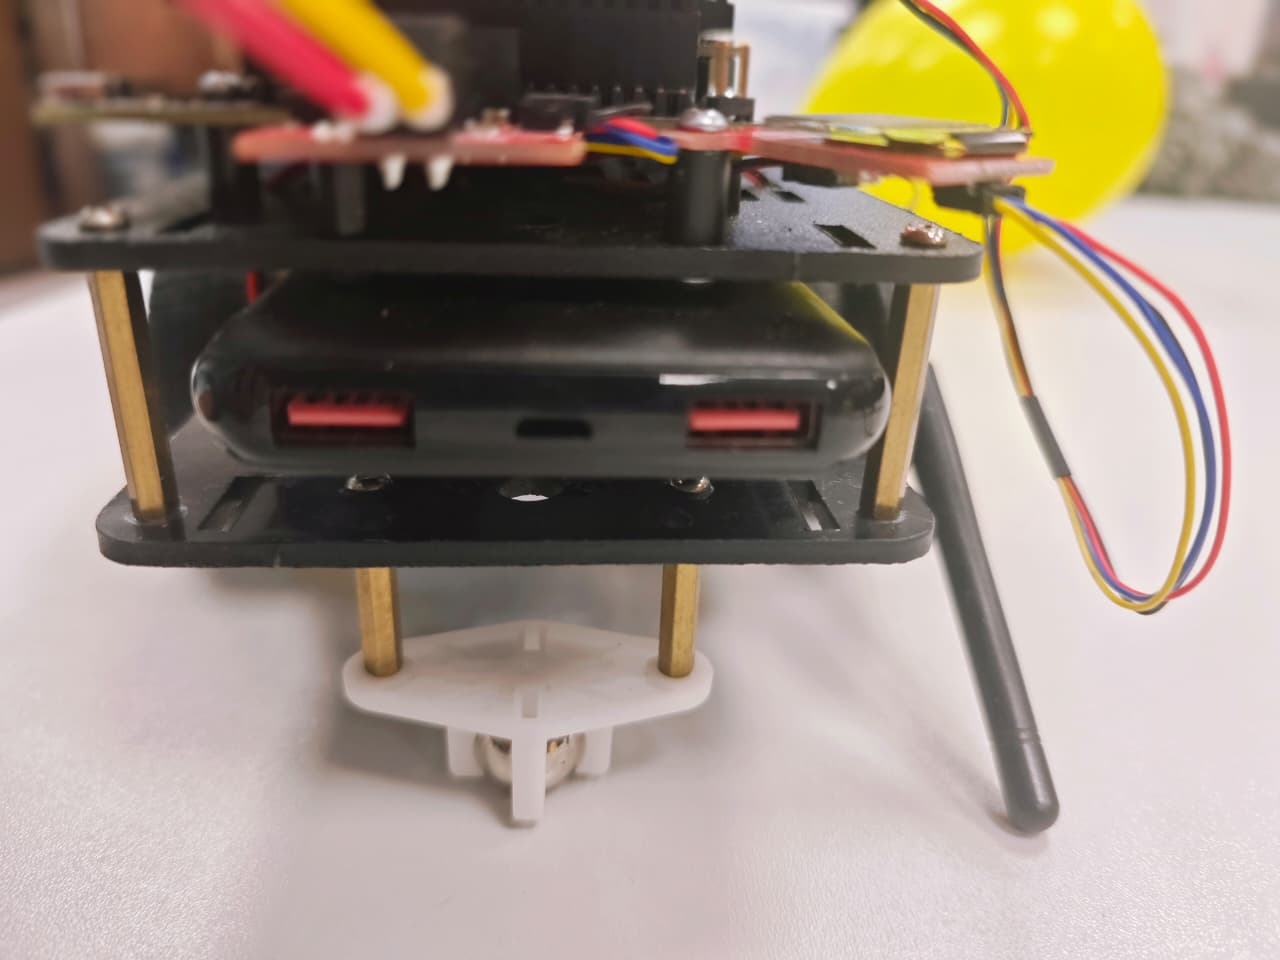
\includegraphics[width=0.7\linewidth]{images/MBBackView}
	\caption{Mobile Robot Rear View}
	\label{fig:mbbackview}
\end{figure}

\begin{figure}
	\centering
	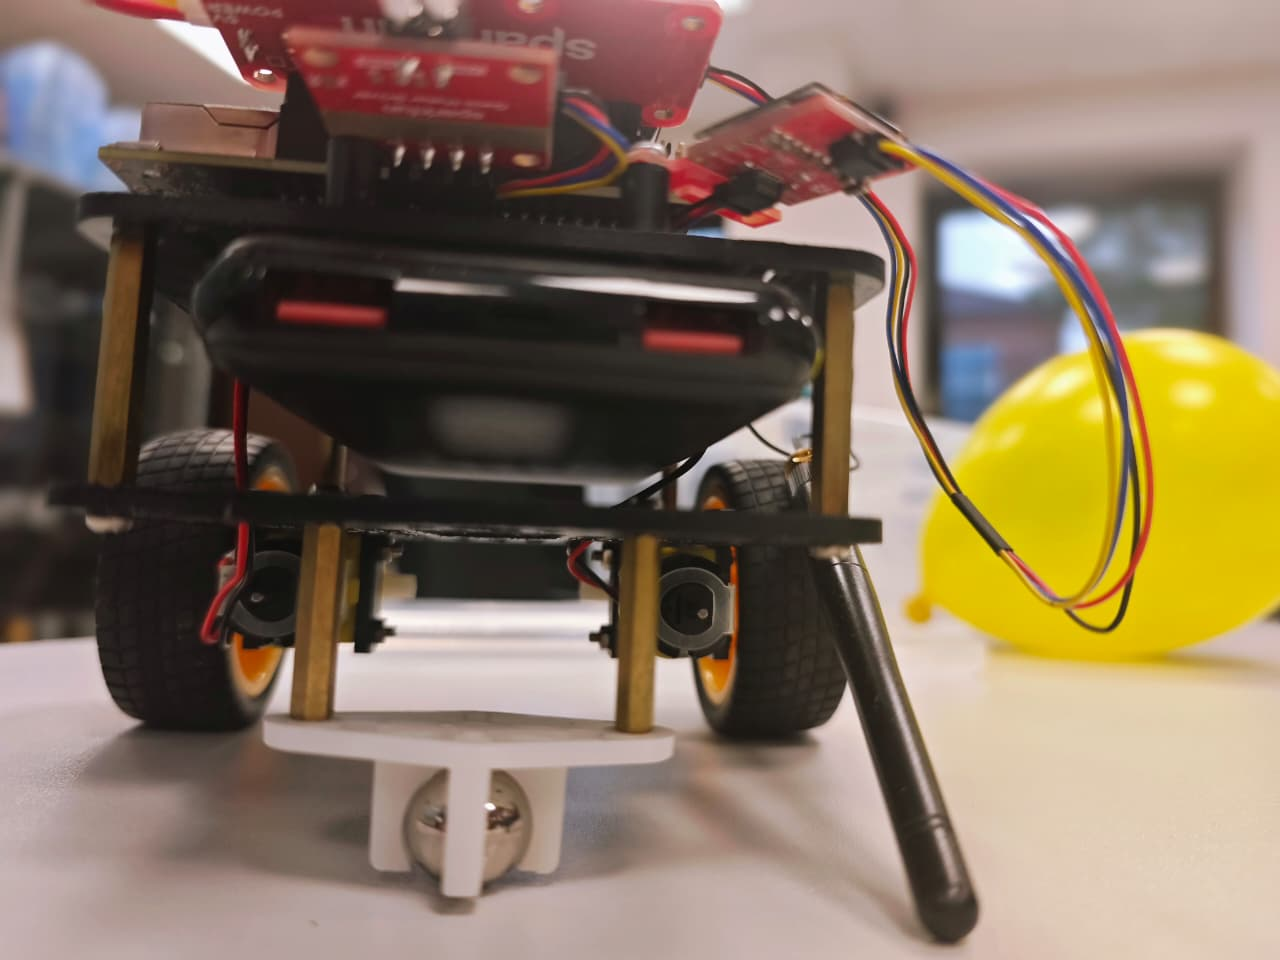
\includegraphics[width=0.7\linewidth]{images/MBWheelball}
	\caption{Mobile Robol Metal Caster Bearing 15.7mm}
	\label{fig:mbwheelball}
\end{figure}
Caster wheel:  
\href{https://www.berrybase.de/adafruit-height-metal-caster-bearing-wheel-stahlkugel-rollenlager-15.7mm-raddurchmesser-20mm-hoch}{Adafruit metal caster} stabilizes the rear of the robot.
}
\STANDARD{Assembly Notes}{
\begin{itemize}
  \item Mount motors at the four corners using provided brackets
  \item Attach caster wheel at rear center for balance
  \item Position Jetson in the middle for weight distribution
  \item Mount cameras at the front for a clear field of view
\end{itemize}
}

%%%%%%%%%%%%%%%%%%%%%%%%%%%%%%%%%%%%%%%%%%%%%%%%%%%%%%%%
%%%%%%%%%%%%%%% PART DETAILS: ELECTRONICS %%%%%%%%%%%%%
%%%%%%%%%%%%%%%%%%%%%%%%%%%%%%%%%%%%%%%%%%%%%%%%%%%%%%%%

\Mysection{Part Details: Electronics}

\STANDARD{Qwiic Boards}{
\textbf{Qwiic pHAT:}  
\href{https://www.berrybase.de/sparkfun-qwiic-phat-fuer-raspberry-pi-v2.0}{SparkFun Qwiic pHAT}  
Provides:
\begin{itemize}
  \item Qwiic connectors for I\textsuperscript{2}C
  \item Clean breakout from 40-pin header
\end{itemize}

\begin{figure}
	\centering
	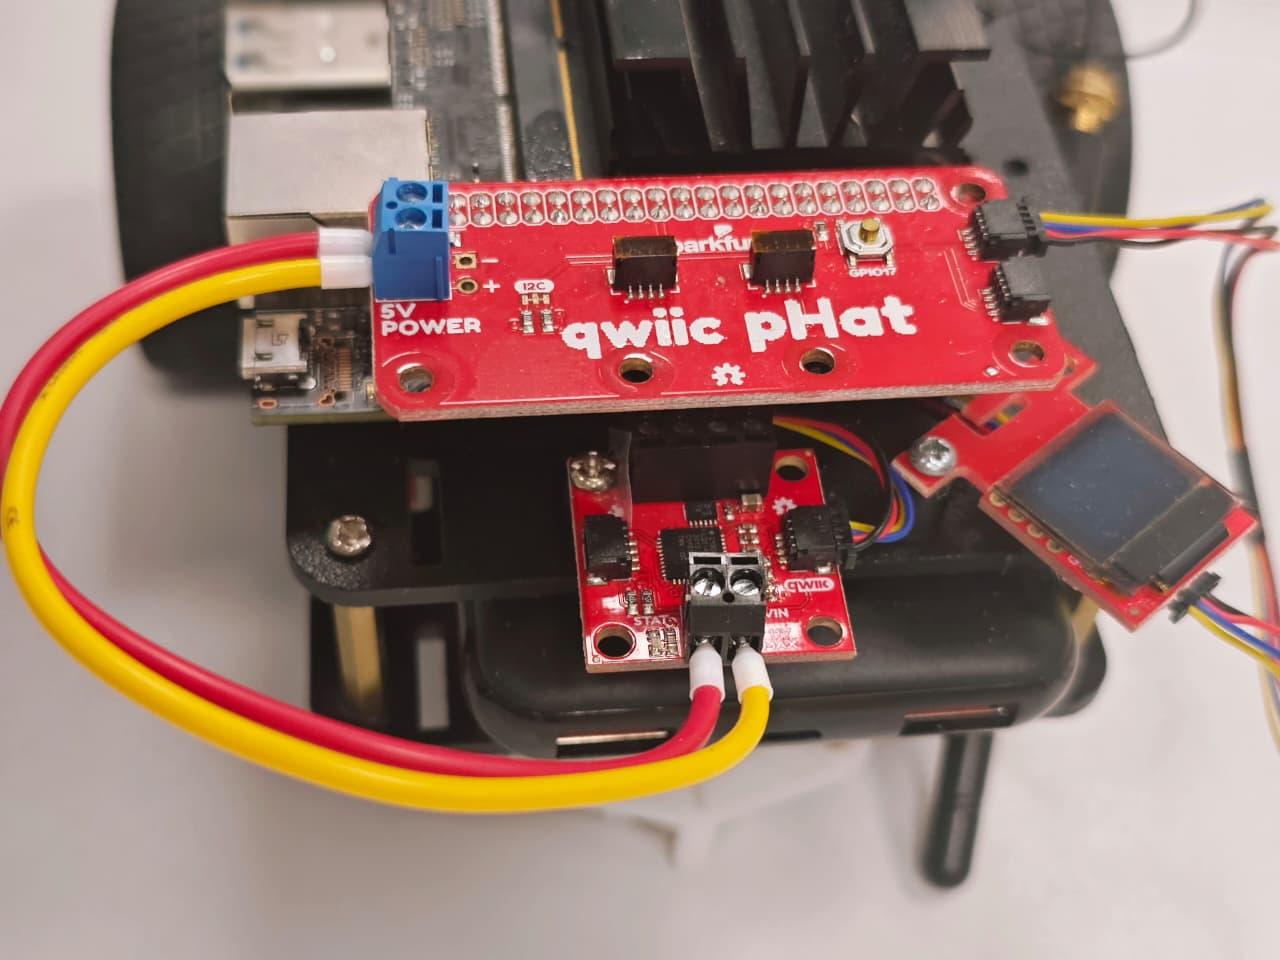
\includegraphics[width=0.7\linewidth]{images/MBqwiicDevBoard}
	\caption{Mobile Robot Qwiic Dev Board}
	\label{fig:mbqwiicdevboard}
\end{figure}

\textbf{Qwiic Motor Driver:}  
\href{https://www.berrybase.de/sparkfun-qwiic-motor-treiber}{SparkFun Qwiic Motor Driver}  
\begin{itemize}
  \item Controls DC motors via I\textsuperscript{2}C
  \item Power input for motor supply
\end{itemize}

\textbf{Qwiic OLED Display:}  
\href{https://www.berrybase.de/sparkfun-micro-oled-breakout-64x48-pixel-qwiic-i2c-10ma-adressierbar-3.3v}{SparkFun Micro OLED}  
\begin{itemize}
  \item Displays status (battery, mode, errors)
  \item I\textsuperscript{2}C-addressable
\end{itemize}
}

\STANDARD{Cables and Antenna}{
\textbf{Qwiic Cables:}  
\href{https://www.berrybase.de/sparkfun-qwiic-kabel-kit}{SparkFun Qwiic Cable Kit}  
\begin{itemize}
  \item Different lengths for flexible routing
  \item Daisy-chain multiple I\textsuperscript{2}C devices
\end{itemize}

\begin{figure}
	\centering
	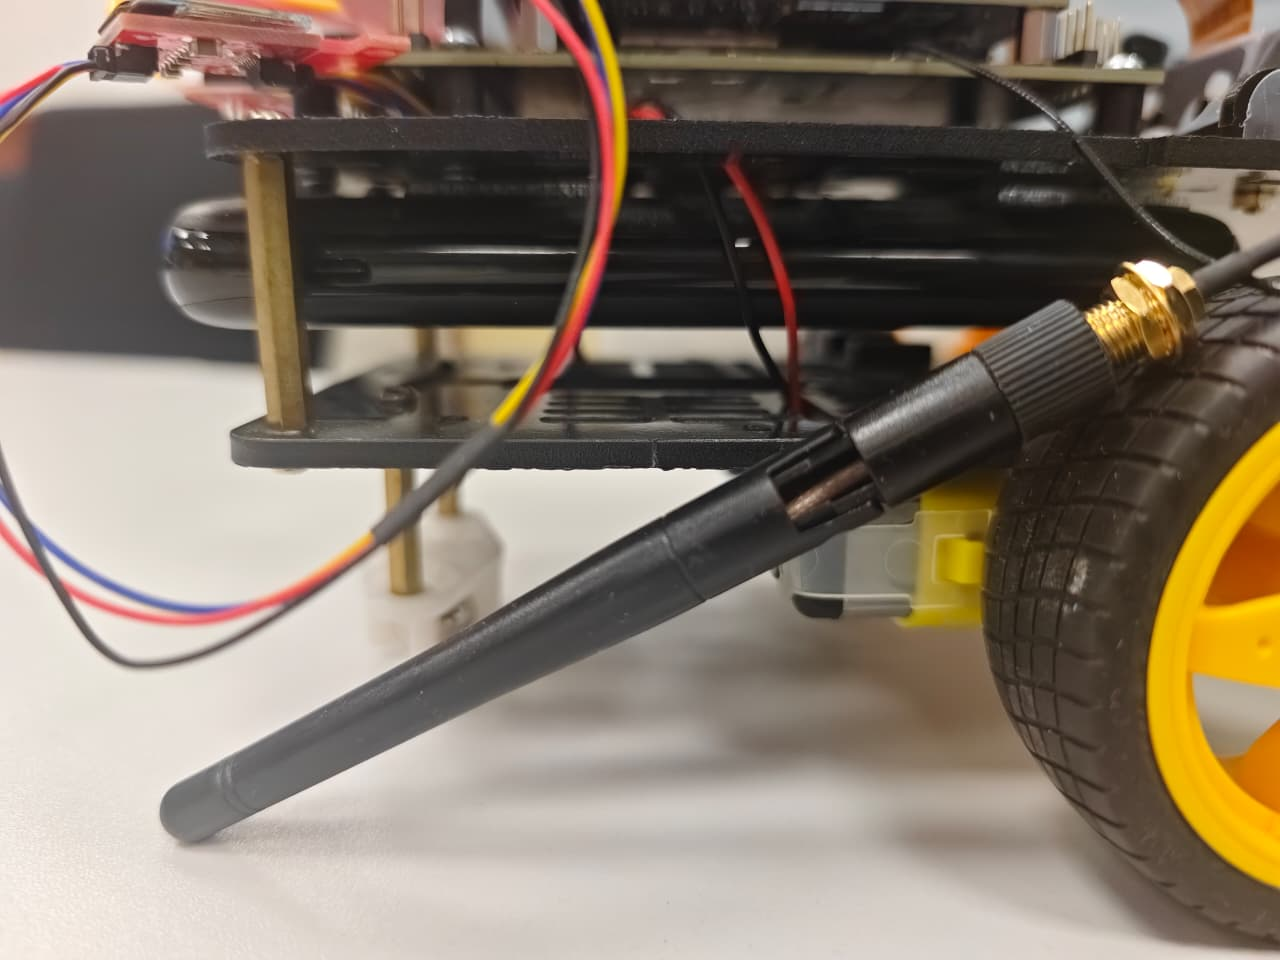
\includegraphics[width=0.7\linewidth]{images/MBAntenna}
	\caption{Mobile Robot Antenna}
	\label{fig:mbantenna}
\end{figure}

\textbf{433 MHz Antenna:}  
\href{https://www.berrybase.de/ism-433-mhz-antenne-sma-2-5-dbi-omnidirektional-flexibel-schwarz}{433 MHz SMA antenna}  
\begin{itemize}
  \item Connects to RF module on the robot
  \item Enables telemetry and remote control
\end{itemize}
}

%%%%%%%%%%%%%%%%%%%%%%%%%%%%%%%%%%%%%%%%%%%%%%%%%%%%%%%%
%%%%%%%%%%%%%%% HARDWARE SETUP & WIRING %%%%%%%%%%%%%%%
%%%%%%%%%%%%%%%%%%%%%%%%%%%%%%%%%%%%%%%%%%%%%%%%%%%%%%%%

\Mysection{Hardware Setup and Wiring}

\STANDARD{Connections Overview}{
\begin{itemize}
  \item Jetson CSI \textrightarrow{} camera ribbon
  \item Jetson 40-pin header \textrightarrow{} Qwiic pHAT
  \item Qwiic pHAT \textrightarrow{} motor driver, OLED via Qwiic cables
  \item Motor driver terminals \textrightarrow{} TT motors on chassis
  \item RF module \textrightarrow{} 433 MHz antenna via SMA
\end{itemize}
}
\STANDARD{Connections Overview Figure}{
\begin{center}
\begin{tikzpicture}
  \node (jetson) [rectangle, draw] {Jetson Nano};
  \node (qwiic) [rectangle, draw, right=3cm of jetson] {Qwiic pHAT};
  \node (mot) [rectangle, draw, below=1.5cm of qwiic] {Motor Driver};
  \node (oled) [rectangle, draw, above=1.5cm of qwiic] {OLED};
  \node (motors) [rectangle, draw, below=1.5cm of mot] {Motors};
  \draw[<->] (jetson) -- (qwiic);
  \draw[<->] (qwiic) -- (oled);
  \draw[<->] (qwiic) -- (motors);
  \draw[<->] (motors) -- (mot);
\end{tikzpicture}
\end{center}
}

%%%%%%%%%%%%%%%%%%%%%%%%%%%%%%%%%%%%%%%%%%%%%%%%%%%%%%%%
%%%%%%%%%%%%%%% CALIBRATION & ODOMETRY %%%%%%%%%%%%%%%%
%%%%%%%%%%%%%%%%%%%%%%%%%%%%%%%%%%%%%%%%%%%%%%%%%%%%%%%%

\Mysection{Calibration and Odometry}

\STANDARD{Camera Calibration}{
\textbf{Goal:} correct lens distortion and obtain camera matrix.

\begin{itemize}
  \item Print a chessboard target and mount it on a flat surface
  \item Capture 20--30 images with different viewpoints
  \item Use an OpenCV calibration script offline
  \item Save intrinsic matrix and distortion coefficients for use in MR.py
\end{itemize}
}

\STANDARD{Wheel Odometry}{
\textbf{Parameters:}
\begin{itemize}
  \item Wheel radius
  \item Wheelbase (distance between left and right wheels)
\end{itemize}

\textbf{Procedure:}
\begin{itemize}
  \item Command robot to drive straight for a known distance
  \item Adjust scaling between motor command and wheel speed
  \item Turn robot in place by 360° and re-center heading
\end{itemize}
}

%%%%%%%%%%%%%%%%%%%%%%%%%%%%%%%%%%%%%%%%%%%%%%%%%%%%%%%%
%%%%%%%%%%%%%%% ROS2 INTEGRATION %%%%%%%%%%%%%%%%%%%%%%
%%%%%%%%%%%%%%%%%%%%%%%%%%%%%%%%%%%%%%%%%%%%%%%%%%%%%%%%

\Mysection{ROS2 Integration}

\STANDARD{ROS2 Node Graph}{
In ROS2, MR.py can be wrapped in a node:

\begin{itemize}
  \item \textbf{Node:} \PYTHON{mobile\_robot\_node}
  \item \textbf{Subscribes:} \SHELL{/cmd\_vel} (geometry\_msgs/Twist)
  \item \textbf{Publishes:} \SHELL{/odom} (nav\_msgs/Odometry)
  \item \textbf{Publishes:} \SHELL{/camera/image\_raw} if desired
\end{itemize}

Conceptual layout:
\begin{center}
\begin{tikzpicture}
  \node (node) [rectangle, draw] {mobile\_robot\_node};
  \node (cmd) [rectangle, draw, left=1.5cm of node] {/cmd\_vel};
  \node (odom) [rectangle, draw, right=1.5cm of node] {/odom};
  \node (img) [rectangle, draw, above=1.5cm of node] {/camera/image\_raw};
  \draw[->] (cmd) -- (node);
  \draw[->] (node) -- (img);
  \draw[->] (node) -- (odom);
\end{tikzpicture}
\end{center}
}

\STANDARD{ROS2 Behavior}{
\textbf{Inside ROS2 node:}
\begin{itemize}
  \item Timer callback runs odometry updates
  \item Subscriber callback updates target wheel speeds
  \item Odometry is published periodically on \PYTHON{/odom}
  \item Motor driver is commanded based on velocity commands
\end{itemize}

In MR.py we implement:
\begin{itemize}
  \item A ROS2 \PYTHON{Node} class wrapping MotorDriver and Odometry
  \item A main entry function \PYTHON{run\_ros2()} that starts the node
\end{itemize}
}

%%%%%%%%%%%%%%%%%%%%%%%%%%%%%%%%%%%%%%%%%%%%%%%%%%%%%%%%
%%%%%%%%%%%%%%% CODE SNIPPETS FROM MR.py %%%%%%%%%%%%%%
%%%%%%%%%%%%%%%%%%%%%%%%%%%%%%%%%%%%%%%%%%%%%%%%%%%%%%%%

\Mysection{Code Snippets and Tests}
\begin{frame}{Overview of MR.py}
	\begin{itemize}
		\item Python3 script for controlling a Jetson-based differential-drive robot.
		\item Supports both:
		\begin{itemize}
			\item \textbf{Standalone mode} (no ROS2 required)
			\item \textbf{ROS2 mode} \PYTHON{(cmd\_vel + odometry)}
		\end{itemize}
		\item Components handled:
		\begin{itemize}
			\item Camera initialization and capture
			\item Motor driver abstraction
			\item Differential-drive odometry
			\item Calibration utilities
			\item Test routines
		\end{itemize}
	\end{itemize}
\end{frame}

%-------------------------------------------------------
\begin{frame}{Camera System}
	\begin{itemize}
		\item Uses OpenCV's \SHELL{VideoCapture}.
		\item Function: \PYTHON{init\_camera(index, width, height)}.
		\item Steps:
		\begin{itemize}
			\item Opens camera at given index.
			\item Sets resolution (default 1280×720).
			\item Returns OpenCV capture object.
		\end{itemize}
		\item Warning printed if the camera fails to open.
	\end{itemize}
\end{frame}

%-------------------------------------------------------
\begin{frame}{Motor Driver Abstraction}
	\begin{itemize}
		\item Class: \PYTHON{MotorDriver}.
		\item Placeholder for Qwiic motor driver (replace later with real hardware API).
		\item Attributes:
		\begin{itemize}
			\item \PYTHON{left\_speed}
			\item \PYTHON{right\_speed}
		\end{itemize}
		\item Methods:
		\begin{itemize}
			\item \PYTHON{set\_speeds(left, right)} – prints motor command.
			\item \PYTHON{stop()} – sets both motors to zero.
		\end{itemize}
	\end{itemize}
\end{frame}

%-------------------------------------------------------
\begin{frame}{Odometry System}
	\begin{itemize}
		\item Class: \PYTHON{Odometry}.
		\item Implements differential-drive kinematics.
		\item Parameters:
		\begin{itemize}
			\item Wheel radius \(r = 0.033\) m
			\item Wheel base \(L = 0.17\) m
		\end{itemize}
		\item Tracks robot pose:
		\begin{itemize}
			\item \(x\) position
			\item \(y\) position
			\item \(\theta\) heading angle
		\end{itemize}
		\item Updates via:
		\[
		v = \frac{r}{2}(w_r + w_l), \quad
		\omega = \frac{r}{L}(w_r - w_l)
		\]
	\end{itemize}
\end{frame}

%-------------------------------------------------------
\begin{frame}{Calibration Routines}
	\begin{itemize}
		\item \textbf{Camera Calibration} (placeholder)
		\begin{itemize}
			\item Uses chessboard images in actual implementation.
			\item Returns identity matrix \(K=I\) and zero distortion.
		\end{itemize}
		\item \textbf{Motor Calibration}
		\begin{itemize}
			\item Runs both motors forward briefly.
			\item Helps verify wiring and direction.
		\end{itemize}
	\end{itemize}
\end{frame}

%-------------------------------------------------------
\begin{frame}{Test Functions}
	\begin{itemize}
		\item \textbf{\PYTHON{test\_motors()}}
		\begin{itemize}
			\item Sweeps motors at speeds: 30, 60, 100, 0.
		\end{itemize}
		\item \textbf{\PYTHON{test\_camera()}}
		\begin{itemize}
			\item Captures one test frame.
			\item Saves as \SHELL{test\_frame.jpg}.
		\end{itemize}
	\end{itemize}
\end{frame}

%-------------------------------------------------------
\begin{frame}{Standalone Mode}
	\begin{itemize}
		\item Does not require ROS2.
		\item Workflow:
		\begin{itemize}
			\item Initialize camera + motor driver + odometry.
			\item Perform calibration tests.
			\item Drive forward with fixed speed.
			\item Print odometry for 20 iterations.
		\end{itemize}
		\item Useful for basic debugging and hardware bring-up.
	\end{itemize}
\end{frame}

%-------------------------------------------------------
\begin{frame}{ROS2 Mobile Robot Node}
	\begin{itemize}
		\item Class: \PYTHON{MobileRobotNode(Node)}.
		\item Subscribes to:
		\begin{itemize}
			\item \PYTHON{/cmd\_vel} (linear + angular velocity)
		\end{itemize}
		\item Publishes:
		\begin{itemize}
			\item \PYTHON{/odom} – robot pose and orientation
		\end{itemize}
		\item Timer callback at 20 Hz:
		\begin{itemize}
			\item Computes wheel velocities.
			\item Updates odometry.
			\item Converts yaw to quaternion.
			\item Sends motor commands.
		\end{itemize}
	\end{itemize}
\end{frame}

%-------------------------------------------------------
\begin{frame}{Entry Point}
	\begin{itemize}
		\item Execution controlled by flag: \PYTHON{USE\_ROS2}.
		\item If \textbf{True}: launches ROS2 node.
		\item If \textbf{False}: runs standalone test mode.
		\item Allows easy switching between development and deployment.
	\end{itemize}
\end{frame}
\STANDARD{Code from MR.py }{

\lstinputlisting[
  language=Python,
  style=mystyle,
  firstline=1,
  caption={Mobile Robot Code}
]{Code/MR.py}
}
\STANDARD{Next Steps}
{
	\begin{itemize}
		\item Follow ROS2 presentation.
		\item Research on Ground Localization. 
		\item Read more about the hardware.
	\end{itemize}
}
